\chapter{Modeling users' behaviors}\label{sec:users-behaviors}

    If we want to infer some information about a huge graph, such as the ones behind the web or Facebook, we usually can't perform our computation directly on the real graph, so we use models of the graph.

    Some properties we usually are interested in when dealing with a network (or a graph) are the following:
    \begin{itemize}
        \item the overall number of nodes,
        \item the average degree,
        \item the number of nodes with a certain degree,
        \item the size of the communities,
        \item the degree distribution.
    \end{itemize}

\section{Erdős–Rényi model}
    
    This is a model for generating random graph, that has many applications due to its simplicity, but doesn't fit real world networks: each node has more or less the same degree, based on a fixed probability, while real networks have a gaussian distribution of the degrees.
    
\section{Preferential attachment}
    
    This is another model for generating random graphs, but it follows the rule ``the rich get richer'', meaning that nodes with higher degree will see their degree becoming higher and higher.
    
    The rule used to build a graph is the following: when you have built a graph with $N-1$ nodes, you add the $N$-th node with an edge that goes from $N$ to a node $i$ chosen accordingly to the following probability:
    \begin{flalign*}
        &\Pr{\text{neighbor of $N$ is $i$}} = \frac{deg(i)}{\sum_{k=1}^{N} deg(k)}&
    \end{flalign*}
    where the denominator is a normalization factor.
    
    There exist many variants of this model, for example with each node creating $k$ edges instead of one, with no self-loop, etc.

    \begin{figure}[h!]
        \centering
        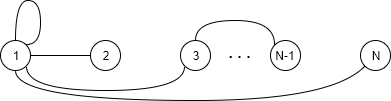
\includegraphics[scale=0.7]{preferential-attach}
        \caption{Preferential attachment}
        \label{fig:pref-att}
    \end{figure}

    The graphs generated by the Preferential attachment model follow a power law degree distribution, like the one observed in many real world networks, indeed, the fraction of nodes of degree $x$ approaches $x^{-3}$.\\
    This characteristic causes that this model fits well with social and biological networks, so it can be used to develop efficient algorithms that actually work in practice.
    
    Now we give a general definition of power law:
    \begin{defn}[Power law]
        A power law is a functional relationship $y = ax^{-c}$ between two quantities, where one quantity varies as a power of the other.
    \end{defn}

    As a consequence of the definition, we get that a power law appears as a line in a log log scale plot, as can be seen in fig. \ref{fig:power-law}.

    \begin{figure}[h!]
        \centering
        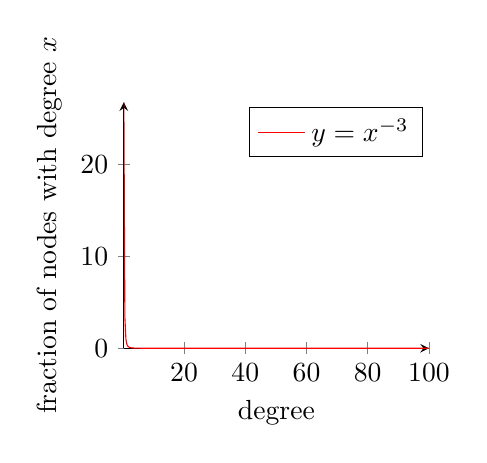
\begin{tikzpicture}
            \begin{axis}[
                width=0.45\textwidth,
                axis lines = left,
                xlabel = degree,
                ylabel = {fraction of nodes with degree $x$},
            ]
            \addplot [
                domain=0:100, 
                samples=300, 
                color=red,
            ]{1/(x^3)};
            \addlegendentry{$y=x^{-3}$}
            \end{axis}
        \end{tikzpicture}
        \hskip 7pt
        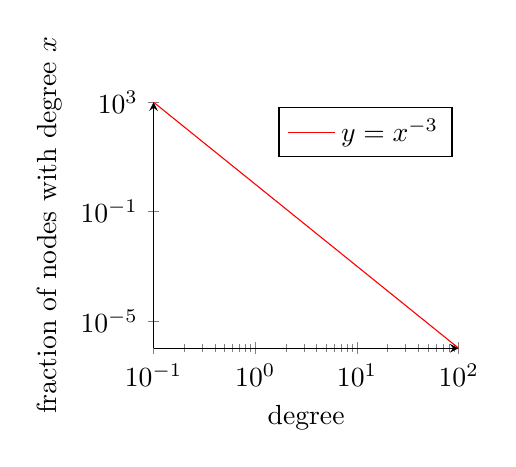
\begin{tikzpicture}
            \begin{axis}[
                width=0.45\textwidth,
                xmode=log,
                ymode=log,
                axis lines = left,
                xlabel = degree,
                ylabel = {fraction of nodes with degree $x$},
            ]
            \addplot [
                domain=0.1:100,
                samples=300,
                color=red,
            ]{1/(x^3)};
            \addlegendentry{$y=x^{-3}$}
            \end{axis}
        \end{tikzpicture}
        \caption{Power law distribution with linear and log log scale}
        \label{fig:power-law}
    \end{figure}
    